\part{Implementation}
\label{pa:implementation}
\chapter{Cytoscape}
\section{Intro}
The \textit{clusterMaker2} documentation for implementing new parts that is not
directly connected with clustering algorithms is non-existing. This part
explains the details about how it was done.

Cytoscape has a cookbook\cite{cytoscape-cookbook} listing a combination of best
practices and tips on how to start developing an app, add menues, panels,
algorithms, color schemes etc.. Instead of following all of these examples, we
have read through the existing code in clusterMaker2\cite{cm2-github} and tried
to structure the code of the contributions in Ranklust to match the structure
already implementet in clusterMaker2. Meaning that for each algorithm
implemented, they will all have a corresponding \textit{Factory} class and a
\textit{Context class}. For the panel that was implemented, it has a pure panel
class with Java Swing\cite{java-swing} settings, a panel task class, create
panel task class and destroy panel task class. % Make UML!

\section{Design}
\begin{figure}[H]
    \caption{Ranklust ranking algorithm relations}
    \label{fig:rank-alg}
    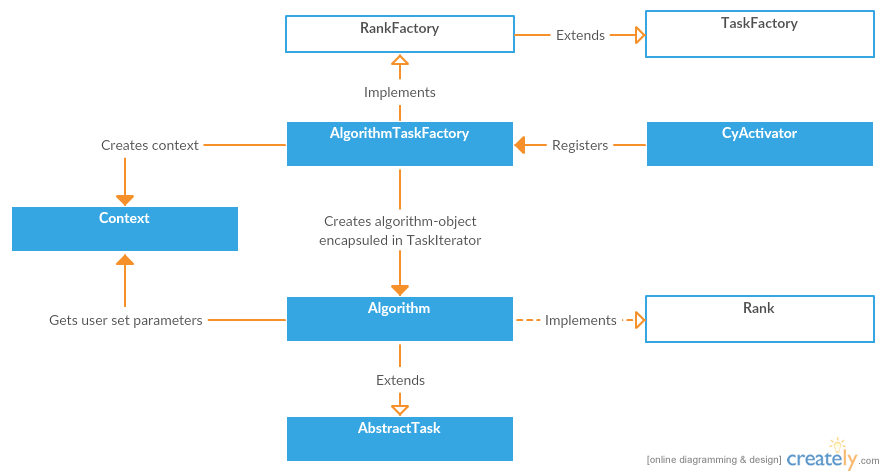
\includegraphics[width=\textwidth]{ranklust-algorithm}
\end{figure}
\begin{figure}[H]
    \caption{Ranklust ranking panel relations}
    \label{fig:rank-panel}
    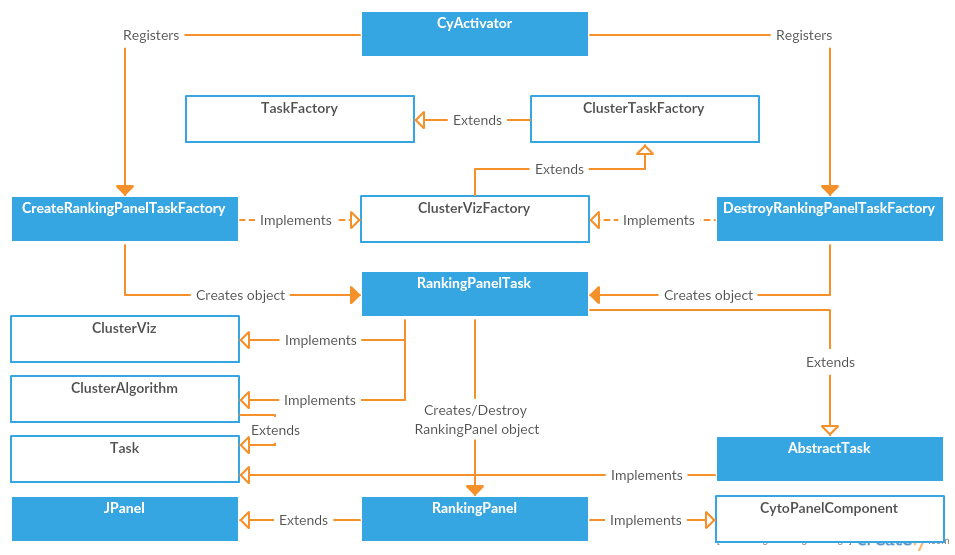
\includegraphics[width=\textwidth]{ranklust-panel}
\end{figure}

\section{Maven and the POM file}
The POM-file has to be updated because libraries connected to the pdf exporting
functionality is outdated. Updating the libraries, imports and the usage of
these libraries in the source code is enough to make the whole project compile.
Also, in order to get the third-party libraries to JUNG\cite{jung} into the
project, the three packages that is being used has to be added to the POM file
and the classes they contain has to be exposed in the OSGi
module\cite{osgi-felix}. Exposing the JUNG classes inside the clusterMaker2 OSGi
bundle could have been avoided if JUNG had OSGi modules in maven repositories,
but there is only 2 out of 3 OSGi ready modules that was needed in this project.
These were the changes needed:

Changed which packages was exported through the OSGi module.

\begin{lstlisting}[language=XML, caption={POM-file OSGi changes}]
<Export-Package>!${bundle.namespace}.*,*;-split-package:=merge-first</Export-Package>
\end{lstlisting}

Added these dependencies

\begin{lstlisting}[language=XML, caption={POM-file JUNG changes}]
<dependency>
    <groupId>net.sf.jung</groupId>
    <artifactId>jung-graph-impl</artifactId>
    <version>2.1</version>
</dependency>
<dependency>
    <groupId>net.sf.jung</groupId>
    <artifactId>jung-algorithms</artifactId>
    <version>2.1</version>
</dependency>
<dependency>
    <groupId>net.sf.jung</groupId>
    <artifactId>jung-api</artifactId>
    <version>2.1</version>
</dependency>
\end{lstlisting}

As seen here, the 3 modules needed is jung-api, jung-graph-impl and
jung-algorithms. Only the first 2 was OSGi ready. An alternative could have been
to create a OSGi ready module of the jung-algorithms module, but taking on the
responsibility for having a module updated at all times is too much for a single
person. However, it could become the clusterMaker2's developers responsbility to
create and update all 3 modules. The last alternative is to find other graph
ranking algorithm libraries like Apache Spark\cite{spark}, thas is OSGi ready.
The reason for not choosing Apache Spark is that it was not discovered until all
of the Java implementation was finished, making it a future goal to reach, at
best.

\section{App registration and java class connections}
First step of registration is to register a \textit{service listener} to the
already existing clusterMaker2 \textit{CyActivator}. Here we describe the name
of java methods in the \textit{clusterManager} class with strings. These two
methods for adding and removing ranking algorithms registers and unregisters the
algorithms to the \textit{App} menu in Cytoscape, making them accessible for the
user through the GUI. Registering a new service listener is a way of keeping the
Ranklust part out of clusterMaker2. Also, creating a standalone plugin at
a later stage will be easier if Ranklust is properly compartmentalized.

% insert code example (lstlistings)

The \textit{RankFactory} class is a java public interface used for each of the
ranking cluster algorithms, HITS, PR, PRWP, MAA and MAM. A class applying the
task factory design pattern is meant to deliver an object of the class it is
related to\cite{factory-design}, and it can return different types of a class
that has the same java superclass\cite{java-superclass}. In this case, each
class implementing the \textit{RankFactory} will only have a single class to
return. The RankFactory class also creates a \textit{Context} class, which binds
information the user can input to the GUI to variables, allowing the algorithm
to gain access to parameter information about the algorithms before they run.

\section{Algorithm}
% Rank interface
\section{GUI}
\subsection{Algorithm menus}
Much of these menus
\subsection{Ranking panel}
The code for the \textit{RankingPanel} is a copy from the existing
\textit{ResultsPanel} in clusterMaker2. The results panel has some extra
information that is removed in the ranking panel. The ranking panel only
displays which clustering and ranking algorithm that was used and the network it
is used on, together with the score of each cluster sorted descendingly, having
the highest ranked cluster at the top. The ranking panel will display in the
same place as the results panel, to the right of the network view.

The panel supports multiple selection of clusters through the \textit{Control}
key on the keyboard, much like its existing behaviour on Windows when selecting
multiple directories or files in the \textit{File Explorer}. Selecting the
clusters in the panel will also select them in the network view, enabling the
user to use other Cytoscape utilities on the nodes/clusters selected, for
example create a new network based on only the selected nodes. The color of the
selected nodes will also change in the network view, when the user selects a
cluster in the ranking panel, providing visual feedback to the user, in order to
make it easier for the user to see where the selected nodes/clusters resides in
the network.

When tasking clusterMaker2 with showing the ranking panel, the color of the
nodes will also change. This is to visualize the rank of each cluster in the
network view to the user. Coloring the highest scoring clusters with red or
green and the lowest scoring with the opposite was the first and easiest
solution. There was made a choice to color the whole cluster according to the
rank it received, instead of individually color nodes according the their
contribution to the clusters rank. The user might be interested in choosing what
suits them best when it comes to this, so it might be implemented a menu for the
ranking panel in the future to best meet the users needs.

Taking color blind people into consideration red and green is not the
best combination. Colors resembling red and green in the form of hot-to-cold
colors that all types of colorblind people can view was therefore a criteria to
be met. A style satisfying these criteria will follow, having the hex value of
te color\cite{color-blindness3}, followed by the RGB value that was calculated
using a site that converts from hex to RGB values\cite{color-blindness2}.
\textit{\#ADD rgb\(170,221,221\)} for a blueish and cold color representing low
score. \textit{\#FEC rgb\(255,248,204\)} represents off-brown color that is a step
warmer than the blueish. The warmest color representing the highest scored
clusters is \textit{\#F99 rgb\(255,153,153\)}. The drawback with this color
combination is with people that has color blindness to the degree where they see
only greyscales. The colors low to high will go from grey to light grey to dark
gray, which does not seem logical. The color style might change if users
experience trouble having these colors representing the cluster ranks. 

\section{State of today}
The pull request\cite{git-pull-request} made from the Ranklust
contribution of this thesis has been accepted\cite{ranklust-accepted}, adding
3750 lines of code and deleting 1051. The changes was distributed across 50
files. The type of files edited ranges from the Maven POM-settings file and
.gitignore to plain Java source code files. Further changes will be made, as the
work on the Ranklust contribution will not end when this thesis is delivered.
One of the most recent changes to the contribution is that the
\textit{PageRankWithPriors} algorithm used to analyze the networks in this
thesis assumes undirected edges because of the
\textit{UndirectedSparseMultigraph} graph used, while for normal use, directed
edges is believed by us to be the most sought after choice. Therefore, the pull
request was hardcoded with directed edges. Choosing between directed and
undirected edges should be up to the users of clusterMaker2 and is on the
TODO-list of futures to implement.

\section{Known bugs}
\subsection{Menu bugs}
\paragraph{Unintentional execution of clustering algorithm}
\begin{enumerate}
    \item Open the clusterMaker2 clustering algorithm menu
    \item Select a clustering algorithm
    \item Exit the menu for the algorithm without running it
    \item Repeat step 1-2 and it results in running the previous algorithm that
        was exited
\end{enumerate}
This was the behaviour before Ranklust contributions was added to clusterMaker2,
so it might be clusterMaker2 or it might be Cytoscape itself. Most likely, the
way clusterMaker2 algorithms is started through its \textit{TaskFactory}'s needs
to be changed, but this is just a hunch and not based on any analysis.

\subsection{Ranking panel bugs}
It is a known bug with the style for node coloring that the ranking panel
causes. The colors in the nodes might flicker when several ranking algorithms
has been run and the colors of each node has changed several times. This is
probably related to the previous color style for the nodes and it will be fixed
in the future.

\chapter{Programming specifics}
\section{Tables vs pure OO}
One thing in particular that deserves to be mentioned is the way networks are
handled. The \textit{CyNode} objects themselves does not contain much. This is
because all of the information is saved in the form of plain cells in a
spreadsheet. This may at first seem like a way to make it easy to show
information to the user, but it is also a way of working more efficient with
network data (insert: reference to working with tables on networks is
efficient). Creating objects with attributes for each node in a huge network
will increase the amount of overhead by a pretty noticeable amount. Working with
all of the information in the way of a spreadsheet with rows and columns
includes a decrease in overhead. A new node is a new row in the node table, so
in relation to building the network structure, it is not a complex abstraction.
The difference comes in when the nodes have several attributes. 

In a table or spreadsheet, attributes can be represented as a single column and
be created once for the whole network, instead of once for each node object
created. This assumes that getting the objects out of the table is possible by
either indexing on a number for arrays, or a unique key for map structures.
The result is both a lookup, insertion and deletion time of O(1). These times is
as low as the Big-O notation goes in terms of speed related to the size of
a collection inside a data structure. So both the creation of objects goes
down, and the retrieval of attribute information is as low as it is possible to
get, when we choose to represent the time by Big-O notation. The only drawback
with this implementation is that there is no current type of wrapper around the
row and column system. So the retrieval of information is not done the most
intuitive way. But this is the way Cytoscape works as a whole, so changing the
way this works can either be done through changing the Cytoscape source code, or
implementing a wrapper as a standalone function inside clusterMaker2 or as
a standalone plugin. In Ranklust, an extension to the existing
\textit{NodeCluster} class was used to keep scoring information about nodes in
clusters.

\section{Changes in existing classes}
\subsection{NodeCluster}
\begin{verbatim}
/**
 * In it's simplist form, a Cluster is a group of nodes that represents the
 * nodes that are grouped together as the result of a clustering algorithm
 * of some sort.  A more complicated form of a cluster could include clusters
 * as part of the list, which complicates this class a little....
 */
\end{verbatim}

This comment is in the NodeCluster class. In the Ranklust implementation,
several attributes and methods has been added to this class. Saving the
temporary state of the scores to the clusters could have been done in the node
and edge-tables in Cytoscape, but it was faster both implementation- and
performance-wise to extend the NodeCluster class. Also, a criteria for extending
this class was that the existing API of this class should not change, in order
to avoid unneccessary changes for other classes in clusterMaker2, that is not
a part of the Ranklust contribution. 

Additions to NodeCluster contains variables representing cluster \textit{score},
\textit{rank} and a \textit{HashMap} from a cluster-node's SUID to its score.
The map and rank variables is part of a previous implementation and can be
removed. Adding node scores to the cluster and normalizing it afterwards.

\textbf{Common responsibilities introduced in Ranklust}

\begin{itemize}
    \item Adding node scores to the cluster (ranking algorithm related)
    \item Normalizing cluster scores for a list of clusters (static method)
    \item Calculating min/max/avg scores for a list of clusters (static method)
    \item Ranking a list of clusters by their score and set their rank
        accordingly (ranking panel related)
\end{itemize}

\subsection{GraphicsExportPanel}
Minor changes were done to GraphicsExportPanel when a new class for handling PDF
documents was introduced. This was the result from the need to change the maven
dependency to use the "com.itext"\cite{itext} repository location instead of
a location from "com.lowagie" because the library was relocated
\cite{lowagie-to-itext}.

\section{New classes}
\subsection{ClusterUtils}
\textit{ClusterUtils} is a new class implemented in the Ranklust contribution.
It is used by every cluster ranking algorithm implemented in Ranklust. To some
degree it has a common responsibility with the \textit{ModelUtils} class from
clusterMaker2. The difference being that ClusterUtils is focused on inserting
scores in tables related to cluster ranks. It also normalizes scores not
directly related to a NodeCluster, but rather a group of \textit{CyNodes}, that
has mapped their SUID in Cytoscape to a score received from a ranking algorithm.

\textbf{Common responsibilities introduced in Ranklust}

\begin{itemize}
    \item Getting cluster attribute based on CyNetwork
    \item Getting ranking attribute based on CyNetwork
    \item Ranking clusters firstly by score, secondly by cluster number
        (assuming a small cluster number is a bigger cluster)
    \item Fetching ranking results based on CyNetwork (ranking panel utility)
    \item Fetching clusters based on CyNetwork (ranking algorithm utility)
    \item Add score to a NodeCluster based on specified attribute column and
        CyRow to get it from
    \item Insert cluster scores into the default node- and edge-tables
    \item A simplified way of creating columns based on a specific column name,
        attribute class, table to create column in and immutability status
\end{itemize}

\section{Handling nodes and edges}
Recipe for working the nodes and edges: The steps are almost equal for
calculating both node and edge scores. How the edges are handled depends on what
direction they have. Are they undirected, directed, or unidirected. In the
current version of Ranklust, \textit{PageRankWithPriors} assumes undirected,
\textit{PageRank} and \textit{HITS} assumes directed. \textit{MAA} adds the
score from the edge to the cluster and \textit{MAM} multiplies the highest score
found as an edge attribute with the current cluster score. MAM and MAA assumes
the score is directed corresponding with source and target nodes in the edge
table of Cytoscape.

\begin{enumerate}
    \item Add score to the cluster
    \item Repeat step 1-2 for every edge
    \item Sort clusters based on rank and create a column to represent the
        cluster score
    \item Create single node score from cluster
\end{enumerate}
